\documentclass{article}


% if you need to pass options to natbib, use, e.g.:
%     \PassOptionsToPackage{numbers, compress}{natbib}
% before loading neurips_2023


% ready for submission
\usepackage[final]{neurips_2023}


% to compile a preprint version, e.g., for submission to arXiv, add add the
% [preprint] option:
%     \usepackage[preprint]{neurips_2023}


% to compile a camera-ready version, add the [final] option, e.g.:
%     \usepackage[final]{neurips_2023}


% to avoid loading the natbib package, add option nonatbib:
%    \usepackage[nonatbib]{neurips_2023}

\usepackage[utf8]{inputenc} % allow utf-8 input
\usepackage[T1]{fontenc}    % use 8-bit T1 fonts
\usepackage{hyperref}       % hyperlinks
\usepackage{url}            % simple URL typesetting
\usepackage{booktabs}       % professional-quality tables
\usepackage{amsfonts}       % blackboard math symbols
\usepackage{amsmath}
\usepackage{nicefrac}       % compact symbols for 1/2, etc.
\usepackage{microtype}      % microtypography
\usepackage{xcolor}         % colors
\usepackage{graphicx}
\usepackage{float}
\usepackage{subfig}

\bibliographystyle{plainnat}


\title{ECEN 757 | Homework 2}


% The \author macro works with any number of authors. There are two commands
% used to separate the names and addresses of multiple authors: \And and \AND.
%
% Using \And between authors leaves it to LaTeX to determine where to break the
% lines. Using \AND forces a line break at that point. So, if LaTeX puts 3 of 4
% authors names on the first line, and the last on the second line, try using
% \AND instead of \And before the third author name.

\author{%
  Muhammed U. Ersoy\\
  M.S. ECEN Student\\
  Texas A\&M University\\
  \texttt{mue@tamu.edu} \\
 }

\begin{document}
\maketitle
\section{In the central server algorithm for mutual exclusion, describe a situation in which two
requests are not processed in happened-before order.}

In the simple \textbf{Central Server} algorithm the server does not keep track of the causality using a logical clock. Since the individual proccesses
communicate with the server directly, the communication is susceptible to asymmetric network delays. In the figure below, we 
see an example where $a \rightarrow b \rightarrow c \rightarrow d$ where $c \rightarrow d$ is $p_2$ requesting permission to enter CS. Even though $p_2$'s request has a causality
relationship with $p_1$'s request ($a \rightarrow c$),the server received and processed $p_1$'s request before due to network conditions. $p_1$ receives the token before $p_2$ which breaks
happened-before order.

\begin{figure}[H]
    \centering
    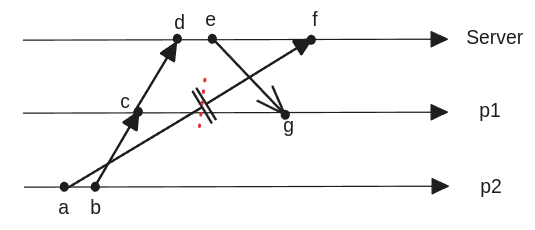
\includegraphics[width=10cm]{mutual_exclusion_me3.png}
    \caption{}
\end{figure}

\section{Adapt the central server algorithm for mutual exclusion to handle the crash failure of any
client (in any state), assuming that the server is correct and given a reliable failure
detector. Comment on whether the resultant system is fault-tolerant. What would
happen if a client that possesses the token is wrongly suspected to have failed?}

If a process currently in CS crashes, then the server could generate a new token and send it to next process
in the queue.
If a process in the queue crashes, then the server could simply pop them from the queue.

If the process in CS is not really crashed (or something malicious is going on) then we could end up with a situation where two
processes try to execute in CS. We could try to mitigate this with versioning. Perhaps this could be embedded into the token such that
when a new token is generated the previous one is invalidated, or the processes could submit a versioning vector for every CS operation (if the datastructure permits this).

\section{Give an example execution of the ring-based algorithm to show that processes are not
necessarily granted entry to the critical section in happened-before order.}

In the ring algorithm, the processes can transmit non-token messages in an arbitrary order. For example, in the figure below the $p_0$ first sends a message to $p_3$ then to
$p_2$. In this case both events $a \rightarrow d$ and $b \rightarrow c$ put their corresponding processes to `awaiting token` state. Since $a \rightarrow b$, for \textit{happened-before} ordering to hold $p_3$ would have to get the token first.
However because the token follows ring ordering, $p_2$ gets to enter CS before $p_3$ which breaks the \textit{happened-before} ordering.

\begin{figure}[H]
    \centering
    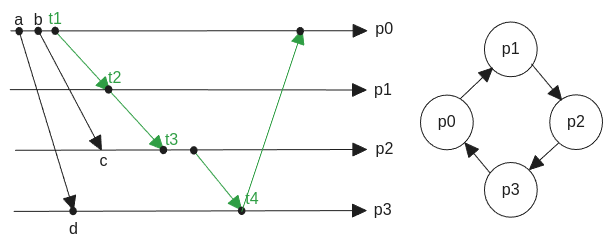
\includegraphics[width=10cm]{ring_algorithm.png}
    \caption{}
\end{figure}
  

\section{In a certain system, each process typically uses a critical section many times before
another process requires it. Explain why Ricart and Agrawala’s multicast-based mutual
exclusion algorithm is inefficient for this case, and describe how to improve its
performance. Does your adaptation satisfy liveness condition ME2?}

Ricart-Agrawala algorithm requires a process to send (multicast) messages to every other machine on the network and wait for \texttt{REPLY} messages from 
all those machines. In total each execution requires $N-1$ messages sent from the requestor, and $N-1$ \texttt{REPLY} messages summing upto $2 (N - 1)$ per CS execution. If a process is currently holding the 
access to CS, but does not need it immediately, it can enter the CS without resending the \texttt{REQUEST} message granted that no other process asked for it. ME2 (liveness) should be preserved, since the process would have to process
the incoming requests in between CS executions.


\section{Suggest how to adapt the bully algorithm to deal with temporary network partitions
(slow communication) and slow processes.}

The following answer was taken from \citet{Borisov}. (\textbf{Reason:} I had thought of the subgroup idea but it didn't feel complete, so I went to check other answers
to see if I am missing something.)

\quote{In case of network partitions, subgroups will be formed. Each subgroup can run Bully algorithm
and elect a coordinator with the highest ID in the subgroup. When the network heals, the subgroups should
merge and elect one coordinator with the highest ID.}

\bibliography{default}
\end{document}


